\begin{exercise}
Schreiben Sie ein Programm, welches für ein gegebenes Runge-Kutta-Verfahren
mit Stabilitätsfunktion $R$ und ein gegebenes Rechteck $Q = \{ z \in \C:
(\Re(z),\Im(z)) \in [a,b] \times [c,d]\}$ diejenigen $z \in Q$ grafisch
hervorhebt, für die $|R(z)| \leq 1$ gilt. \\
Testen Sie dieses Programm mit bereits bekannten expliziten und impliziten
Runge-Kutta-Verfahren. Verwenden Sie unter anderem die Verfahren aus Remark 4.25
und Definition 4.31. Welche Rechtecke $Q$ sind interessant?
\end{exercise}
\begin{solution}
\begin{figure}
    \centering
    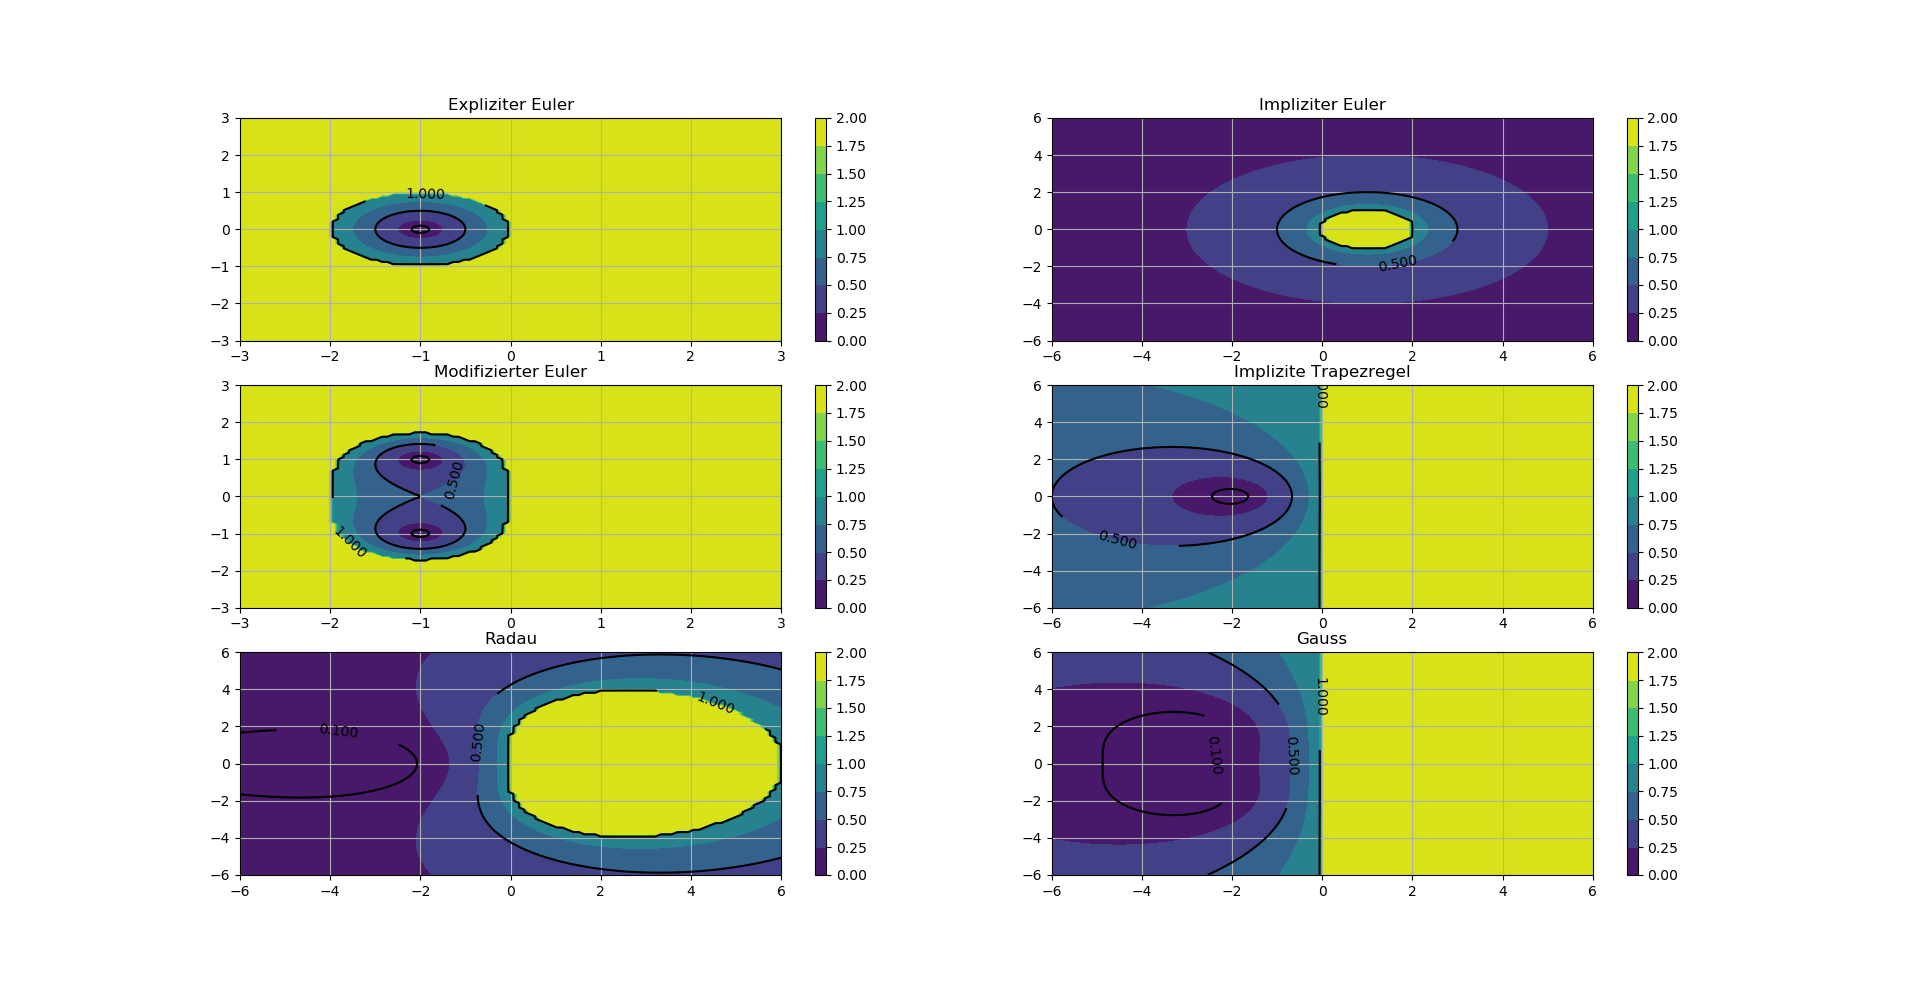
\includegraphics[width=\linewidth]{plot30.png}
\end{figure}
\end{solution}
